\chapter{Tool for automated evaluation}
\label{cha:tool}

\section{Introduction}
\label{sec:tool-introduction}
In the previous chapter we have shown that different integration strategies do make a difference for the performance of the resulting model. In order to facilitate future research on this topic, we have developed a tool that allows anyone to very easily compute all the integrated models and compare them.
\section{Technologies}
\label{sec:tool-technologies}
To develop this tool we needed a programming language that provided a lot of support for statistical algorithms, and we also wanted to create a very user-friendly interface to make an abstraction of the underlying machine learning methods.
\subsection{The R language}
The language we used to create the tool is R. R is a very popular language for statistical research as it provides many state-of-the-art algorithms in statistics. R has a huge repository with packages for all kinds of purposes. The package that we used to compute models is glmnet\cite{glmnetvignette}. It is developed by researchers at the Stanford University and provides very fast implementations to compute the generalized linear models explained in chapter \ref{cha:glm}. 
\subsection{Web interface}
I wanted to offer a very easy-to-use interface to the application. Therefore we chose to work with shiny\cite{shiny}. Shiny is a framework for R that allows you to create a web-based front-end (using html, css, javascript, ...) that can also run R code in the back-end. This allows the creating of very interactive web applications that can run the powerful statistical analyses available in R.
\section{Demonstration}
\label{sec:tool-demonstration}
The tool is divided into three sections: an input section where the user can upload their datasets, a section that computes and evaluates models for each dataset individually, and an integration section where all of the integrated models, explained in chapter \ref{cha:integration}, can be computed and evaluated.
\subsubsection{The input tab}
The input tab allows the user to either use a preloaded dataset or upload their own datasets to the application. It is possible to define multiple dependent variables in one file, the tool then gives you the option to select which variable has to be modeled. \\ \\
When datasets are uploaded, the tool gives a small overview of the dimensions of each dataset so the user can verify everything works correctly. Figures \ref{fig:tool-input} and \ref{fig:tool-input2} show the input page where a user has uploaded some datasets.
\begin{figure}
	\centering
	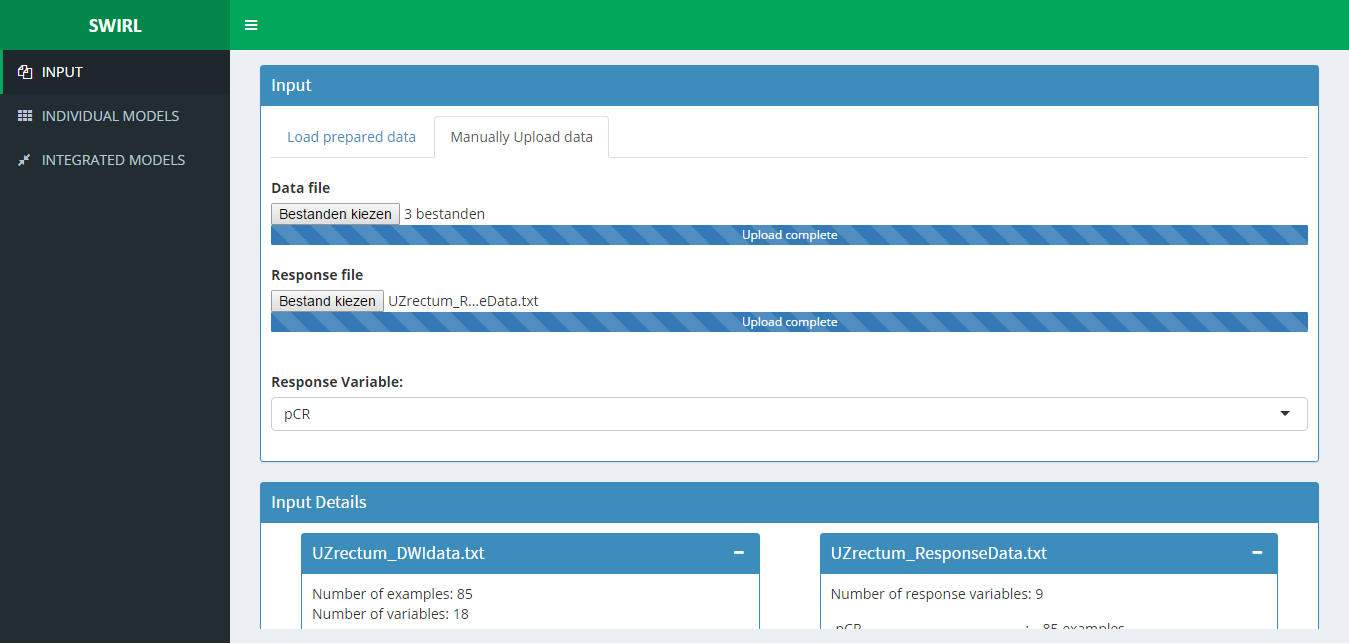
\includegraphics[scale=.3]{images/tool_input_1}
	\caption{The input tab of the tool}
	\label{fig:tool-input}
\end{figure}
\begin{figure}
	\centering
	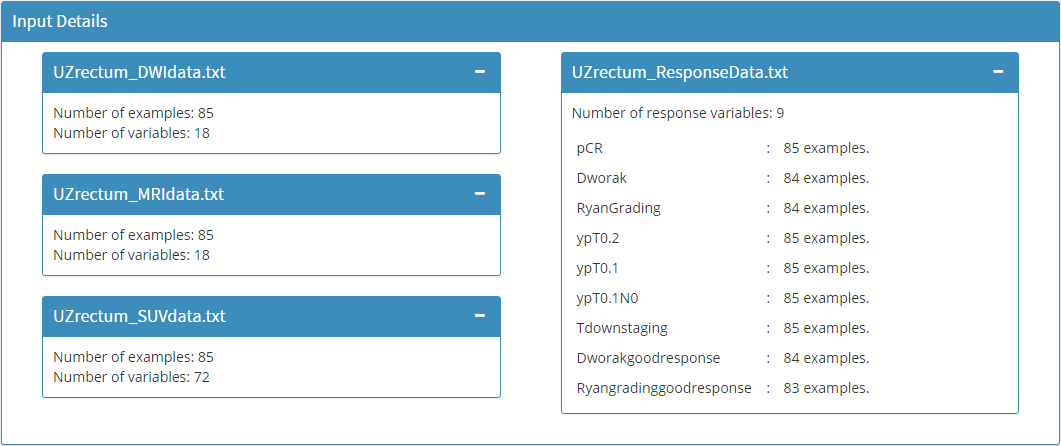
\includegraphics[scale=.4]{images/tool_input_overview}
	\caption{Example input overview. The boxes on the left show explanatory variable dataset dimensions, the box on the right shows the possible dependent variables.}
	\label{fig:tool-input2}
\end{figure}
\subsubsection{The individual models tab}
Once a user has uploaded their datasets they can compute a model for each dataset individually. The tool will give a concise overview of the model parameters for each model, and show an evaluation of the model. In case of logistic regression, the evaluation would be a ROC curve (explained in section \ref{sec:evaluation-logisticregression}). Notice that the evaluation is interactive: the user can use the slider to see the performance metrics for different thresholds. Figure \ref{fig:tool-model} shows an example model description. Figure \ref{fig:tool-roc} shows an example ROC curve.
\begin{figure}
	\centering
	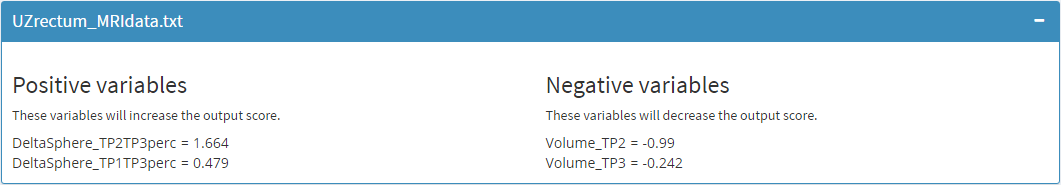
\includegraphics[scale=.4]{images/tool_model_mri}
	\caption{An example model description showing the coefficients for the variables in the model separated by their sign.}
	\label{fig:tool-model}
\end{figure}
\begin{figure}
	\centering
	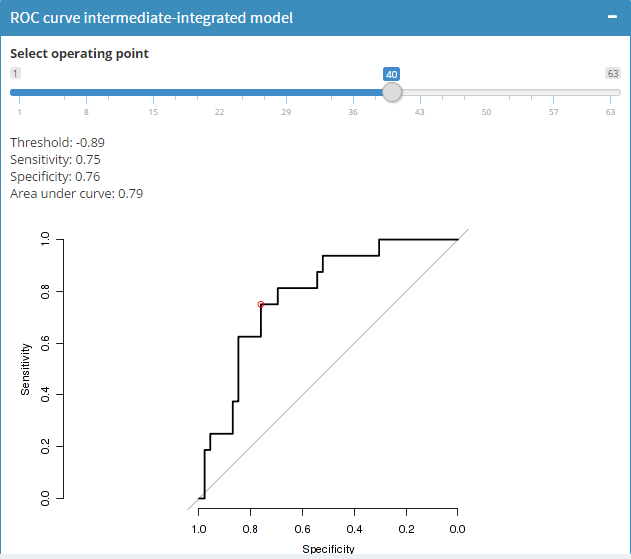
\includegraphics[scale=.65]{images/tool_auc}
	\caption{An example interactive ROC curve. The slider on top allows the user to vary the threshold. The plot interactively adjusts itself to the chosen threshold.}
	\label{fig:tool-roc}
\end{figure}
\subsubsection{The integration tab}
The integration tab is the most important part of the application, as it allows the user to compute and evaluate integrated models for their datasets. The integration tab is further split up into early-, late- and intermediate integration tabs. Each tab allows the user to compute and evaluate its respective integration method. The results will look exactly the same as shown for the individual models tab, as can be seen on figures \ref{fig:tool-model} and \ref{fig:tool-roc}.

\section{Conclusion}
\label{sec:tool-conclusion}
To make further research easier we have made an interactive web-based tool. The tool allows users to compute and evaluate all integration strategies explained earlier. It currently supports logistic regression models and cox proportional hazard models. The back-end uses the statistical language R and the glmnet package to compute the models. The front-end is purely web-based and this is made possible by the Shiny framework.

%%% Local Variables: 
%%% mode: latex
%%% TeX-master: "thesis"
%%% End: 
